\chapter{Results}

In this chapter we will go over the results we obtained by testing our methods.

In the first section we will show the results of training the EfficientPose network on our datasets, and subsequent observations. In the second section we test the performance of our semantic meaning extraction strategy. Finally, in the third section we show how effective our overall system is in a real-world robotics application.

\section{Model Training Results}

In this section we will show the results of training the EfficientPose network on the three datasets presented in the previous chapter: the fully rendered dataset representing an M6x30 screw, henceforth referenced as "ScrewDataset", the augmented reality dataset representing a set of screws, henceforth "ScrewPose", and the augmented reality dataset representing the set of buttons and boards, henceforth "ButtonPose".

\begin{figure}[htp]
    \subfloat[Evolution using ScrewDataset for training.]{
        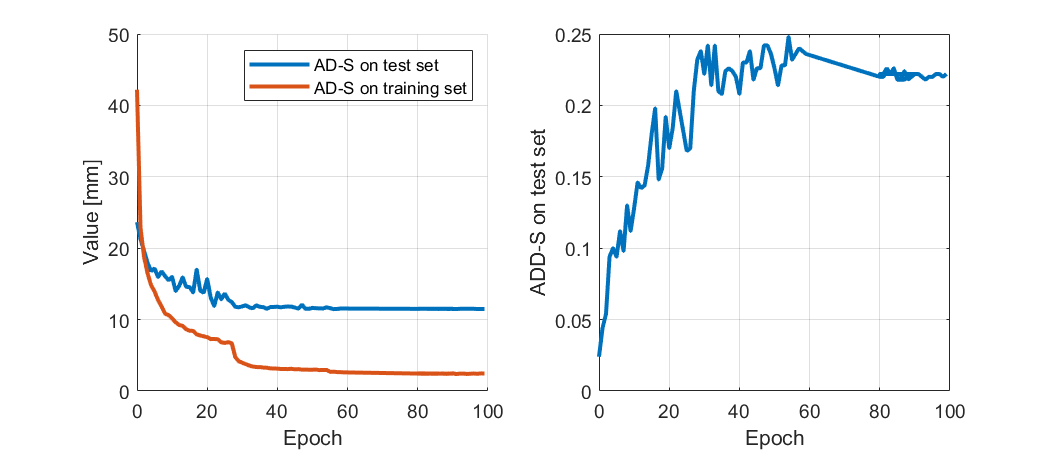
\includegraphics[width=0.7\textwidth]{screwdataset_training.png}
    }

    \subfloat[Evolution using ScrewPose for training.]{
        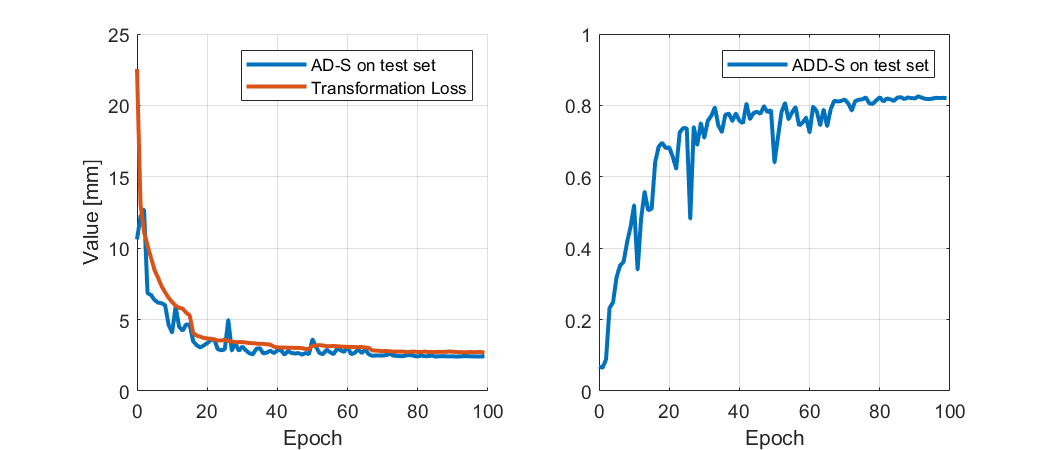
\includegraphics[width=0.7\textwidth]{screwpose_training.png}
    }

    \subfloat[Evolution using ButtonPose for training.]{
        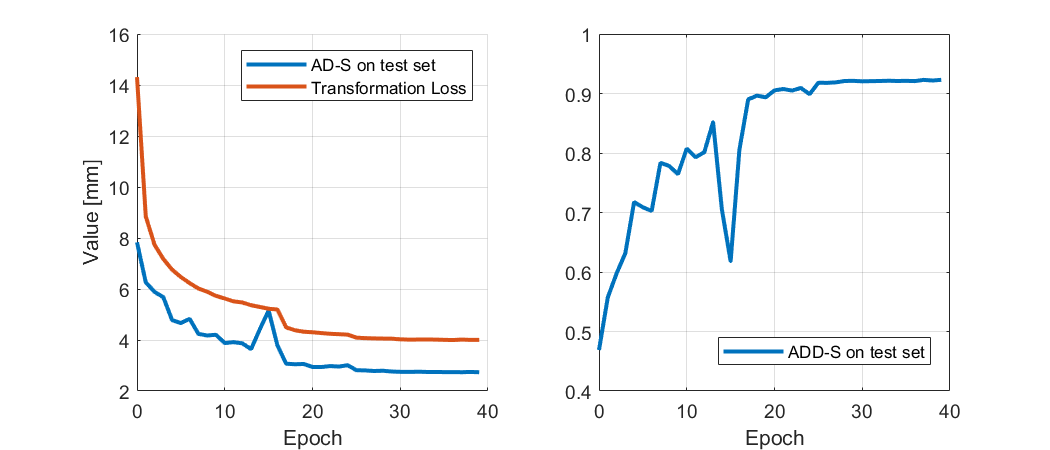
\includegraphics[width=0.7\textwidth]{buttonpose_training.png}
    }

    \caption{Training progress for EfficientPose on the ScrewDatset, ScrewPose and ButtonPose datsets, represented as the evolution of the AD-S and ADD-S metrics in evaluation for each epoch.}
    \label{fig:training_progress}
\end{figure}

We will then be comparing these results with those obtained by EfficientPose on other datasets, namely LINEMOD for single object estimation and Occlusion-LINEMOD for multi-object estimation.

The evolution of the loss and ADD-S metrics during training for these three datasets is shown in figure \ref{fig:training_progress}. As we can see, the model's performance gradually improves over the training period, eventually stabilizing at a plateau for all three datasets. Also visible is the effect of the learning rate reduction, which has visible results when appiled.

As for training results, visible in figure \ref{training_results}, we will examine them independantly for each dataset below.

On ScrewDataset, after 100 epochs of training the model has a final ADD of 22.20\%, with a peak value obtained during training of 24.8\%, much lower than the 97.35\% with $\phi=0$ reported by EfficientPose on LINEMOD. We can hypothesize that the reason for this performance gap is that the rendered dataset is much more difficult than LINEMOD, since we are dealing with a very small, symmetric object hidden inside a chaotic, colorful background with widely differing light conditions. Another serious issue with this dataset is that the model is not able to bridge the reality gap: while testing in real-life scenarios, it failed to identify the screw in most conditions, let alone produce accurate estimations. This means that it generalises poorly outside of the simulated environment, making it essentially unuseable in real world applications.

On the flip side, the ScrewPose datset obtainined an average ADD-S of 82.05\%, which is better than EfficientPose's 79.04\% with $\phi=0$ on Occlusion-LINEMOD, and comparable to its 83.98\% with $\phi = 3$. This is a good result considering that the objects for our dataset are smaller, symmetric and all visually similar. Even though the Occlusion dataset is notoriously challenging, this anyways demonstrates the good performance of our own dataset.

\begin{figure}[htp]
    \subfloat[ScrewDataset.]{
        \begin{tabular}{|c||c|c|c|}
            \hline
            Object & AP & AD-S [mm] & ADD-S \\
            \hline \hline
            M6x30 & 0.9675 & 11.4921 & 22.20\% \\
            \hline
        \end{tabular}
    }

    \subfloat[ScrewPose.]{
        \begin{tabular}{|c||c|c|c|}
            \hline
            Object & AP & AD-S [mm] & ADD-S \\
            \hline \hline
            M6x30 & 0.9399 & 2.1434 & 82.30\% \\
            M8x16 & 0.9538 & 1.9988 & 67.54\% \\
            M8x25 & 0.9645 & 2.1179 & 85.07\% \\
            M8x50 & 0.9880 & 3.4482 & 93.30\% \\
            \hline \hline
            Average & 0.9615 & 2.4271 & 82.05\% \\
            \hline    
        \end{tabular}
    }
    
    \subfloat[ButtonPose.]{
        \begin{tabular}{|c||c|c|c|}
            \hline
            Object & AP & AD-S [mm] & ADD-S \\
            \hline \hline
            2-slot & 0.9990 & 3.5420 & 99.90\% \\
            3-slot & 0.9985 & 3.9304 & 99.85\% \\
            red button & 0.9260 & 1.9825 & 86.01\% \\
            arrow button & 0.9349 & 2.0497 & 86.05\% \\
            safety button & 0.9962 & 2.6053 & 98.01\% \\
            unknown button & 0.9561 & 2.4757 & 82.95\% \\
            \hline \hline
            Average & 0.9685 & 2.76 & 92.13\% \\
            \hline    
        \end{tabular}
    }

    \caption{Evaluation of the Average Precision, Average Symmetric Distance, and ADD-S metrics on the ScrewDataset, ScrewPose and ButtonPose datasets after training.}
    \label{training_results}
\end{figure}

\begin{figure}[htp]
    \subfloat[ScrewPose.]{
        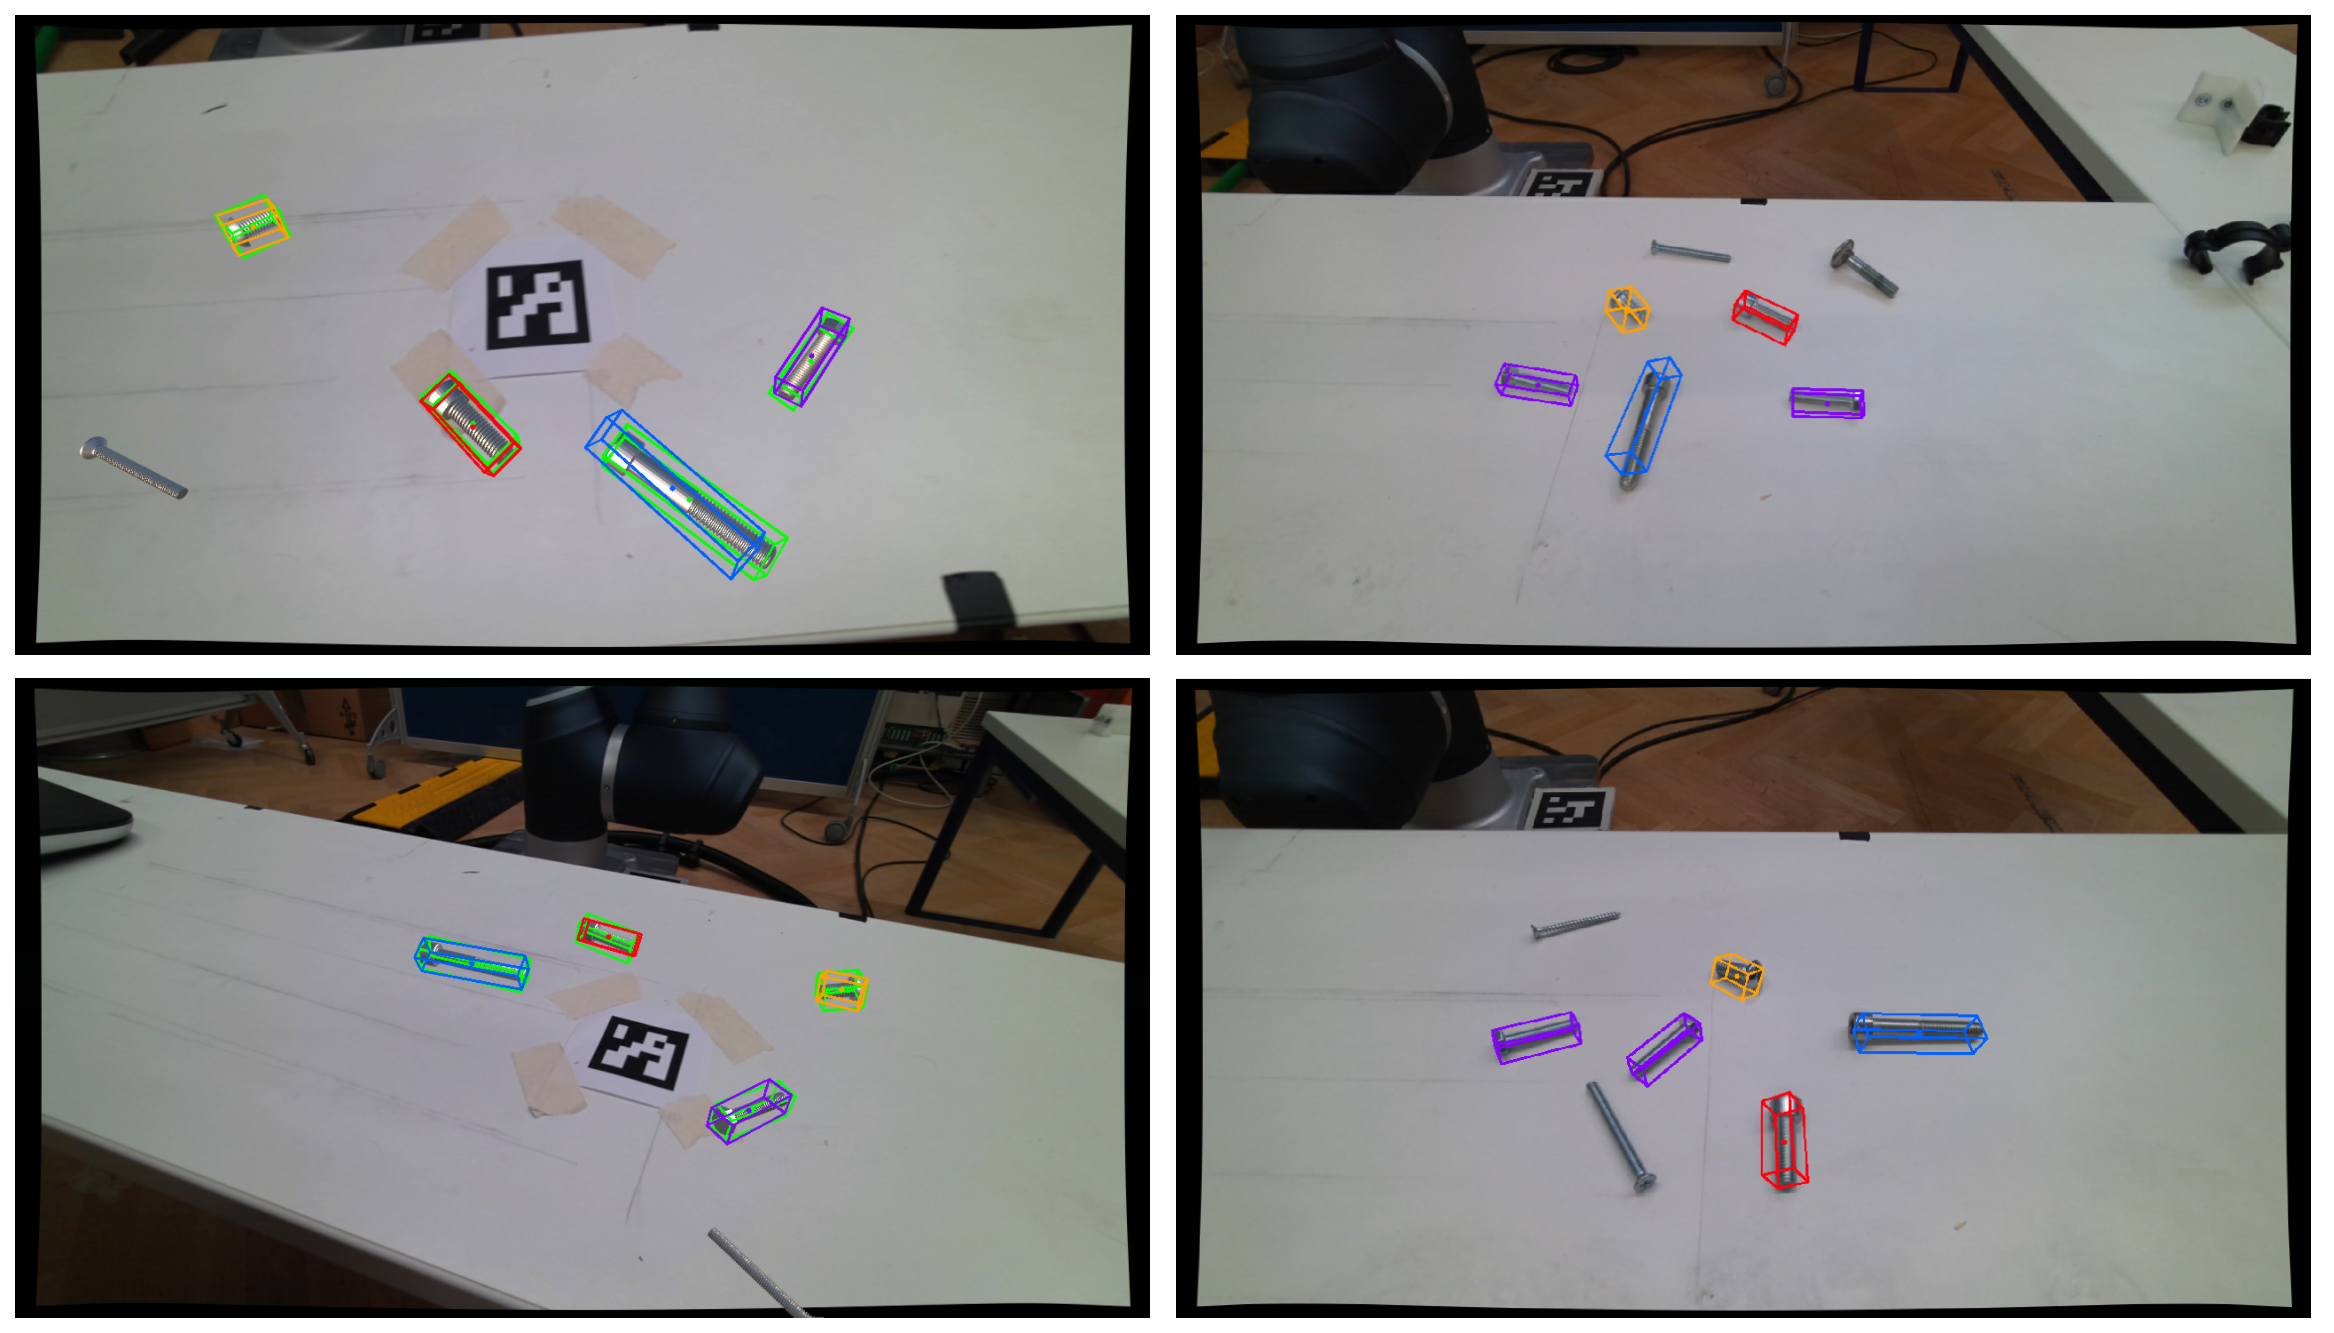
\includegraphics[width=\textwidth]{screwpose_inferencing.png}
    }

    \subfloat[ButtonPose.]{
        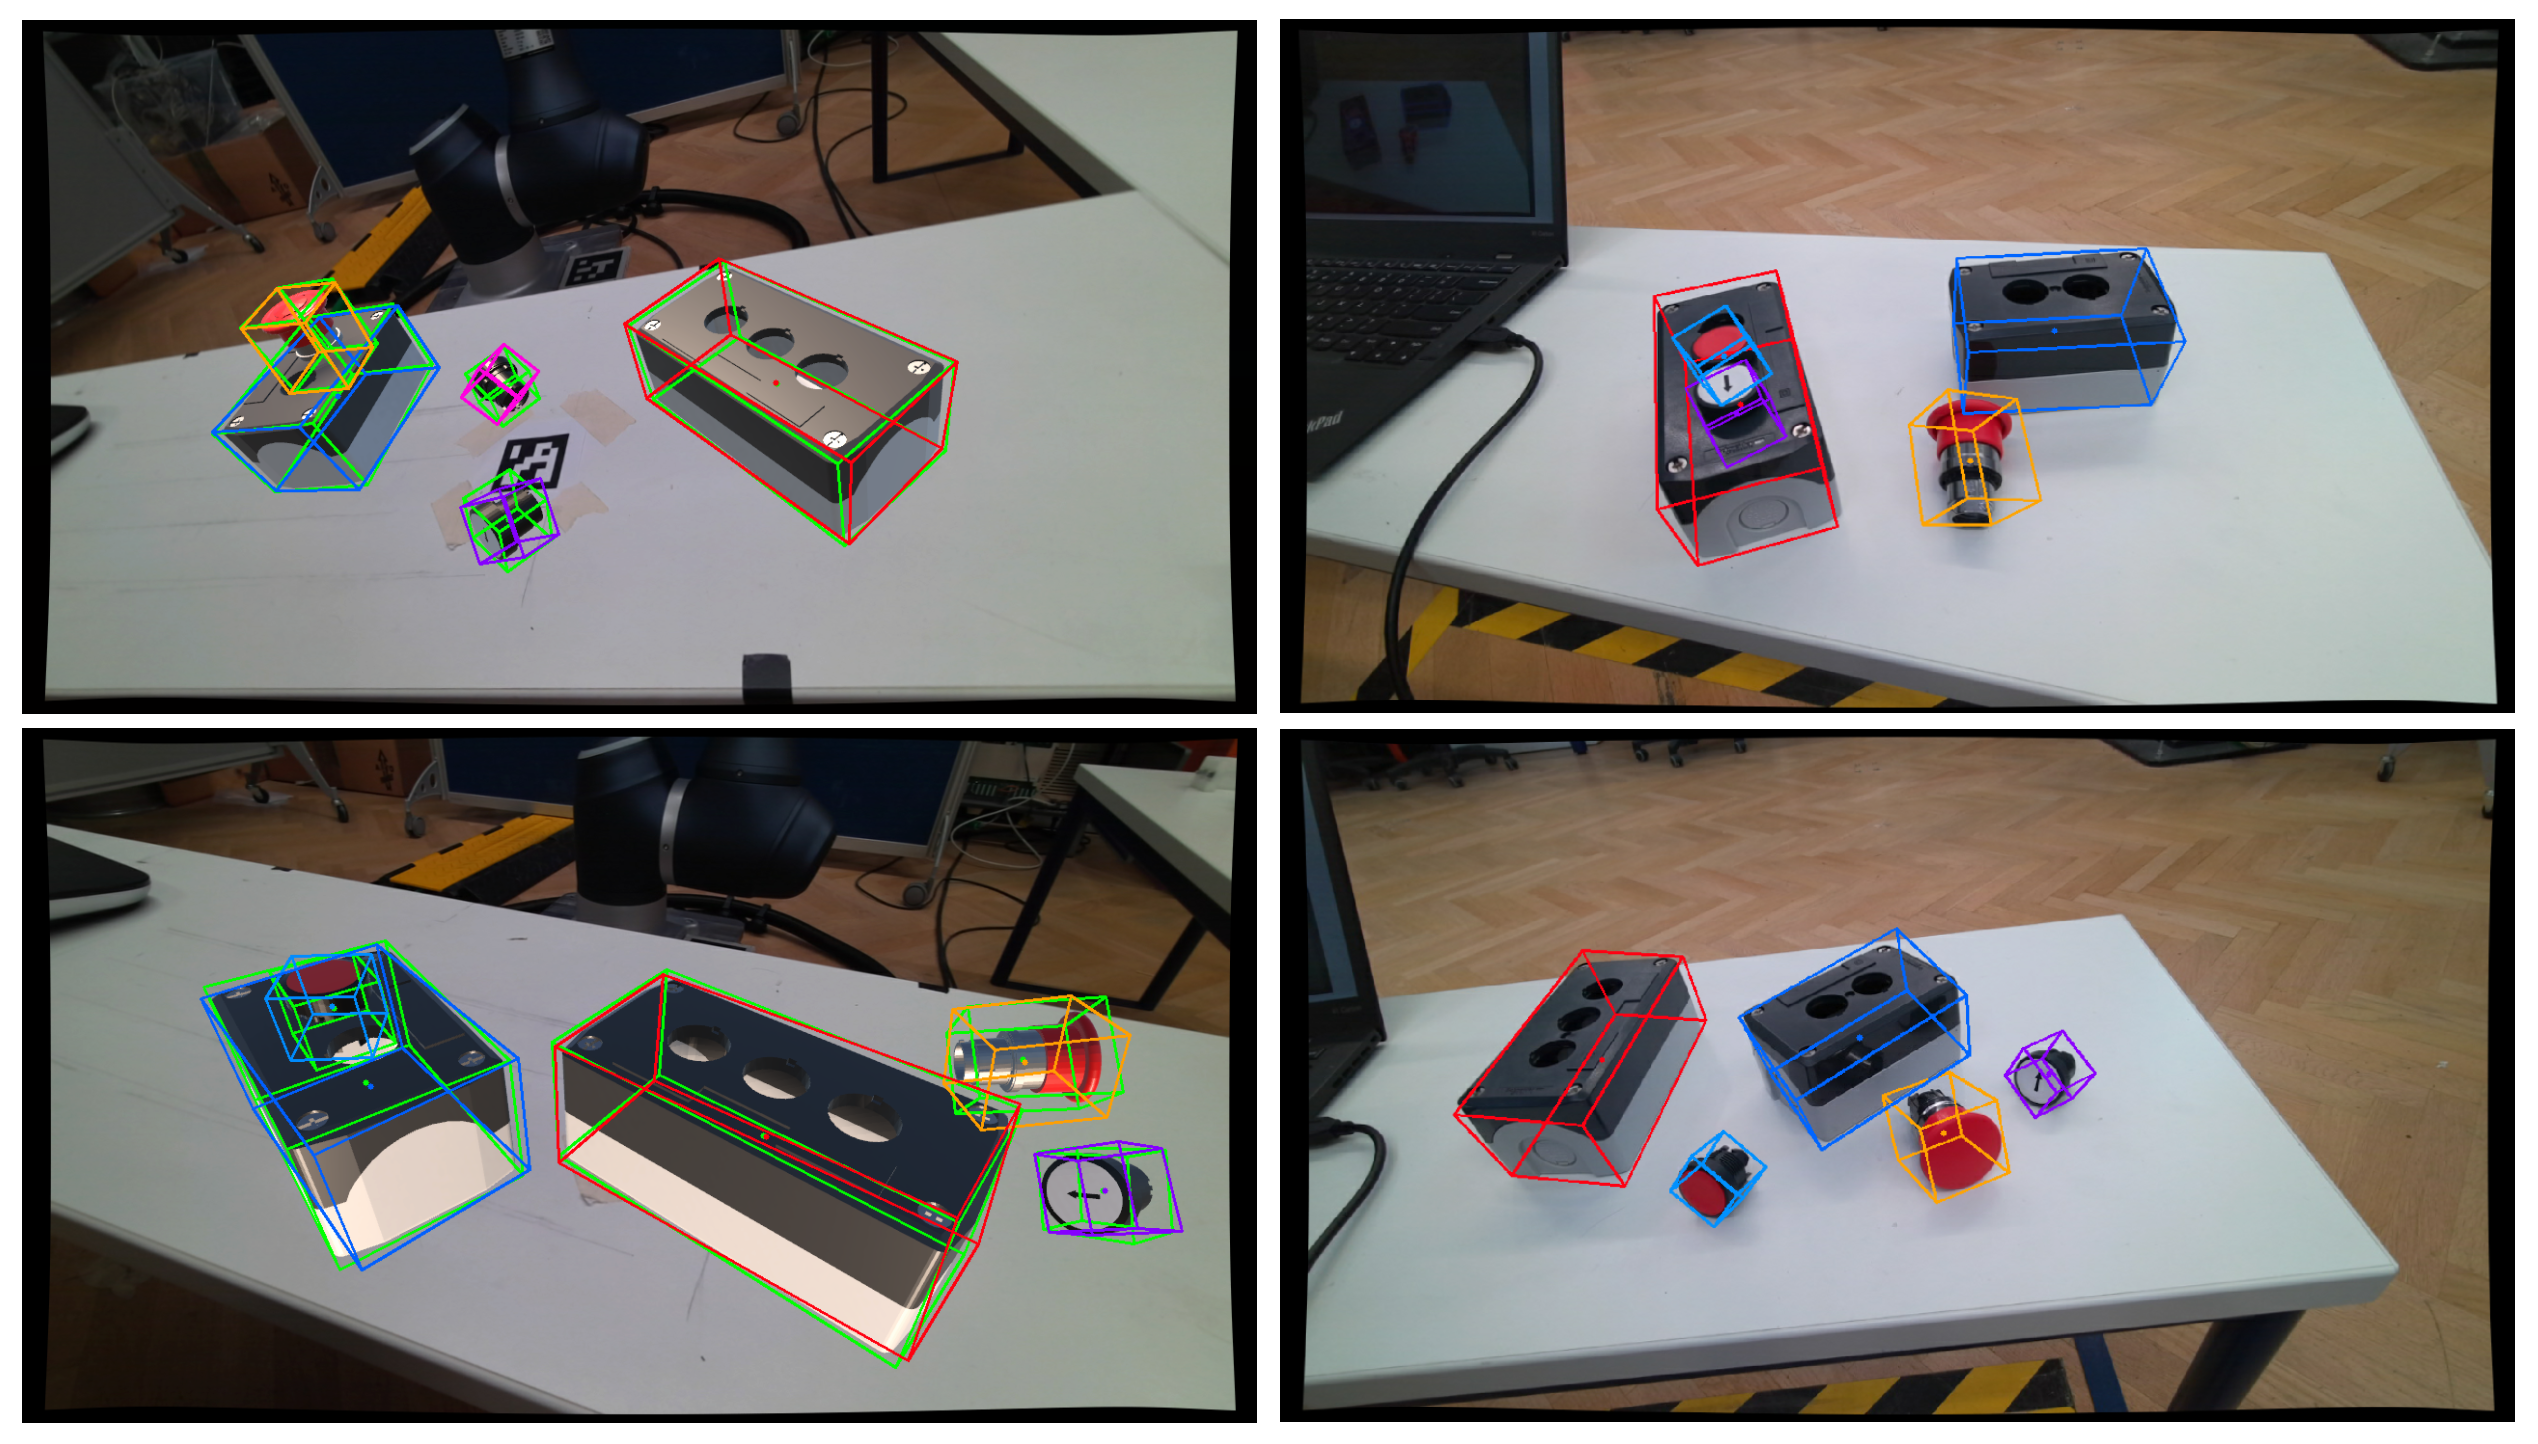
\includegraphics[width=\textwidth]{buttonpose_inferencing.png}
    }

    \caption{Images displaying pose estimations from the network for the ScrewPose and ButtonPose datasets. The left images are part of evaluation and display ground truths with green bounding boxes, the right ones are captures from a real camera in the testing environment.}
    \label{fig:inferencing}
\end{figure}

Finally, training on the ButtonPose dataset resulted in optimal performance for the boards, reaching over 99\% ADD-S and AP for both. The larger safety button also obtained great results, with a 98\% ADD-S, while the other buttons achieved more middling performances, but still better than the Occlusion-LINEMOD benchmark, showing that our approach is valid for more object sets.

The ScrewPose and ButtonPose datasets were also able to generalise to real-life conditions without noticeable losses in performance, as can be observed in figure \ref{fig:inferencing}.

\subsection{Impact of object dimensions and distance}

One noticeable result we observed after training was the impact that physical dimensions have on the final performance of the model for each object. Namely, larger and closer objects have much better performance than smaller and further objects. This is immediately noticeable in the ScrewPose dataset, where the larger M8x50 screw obtained the best results and the M8x16 obtained the worst.

To show how extreme these differences can be, we trained two additional models using new datasets based on the ButtonPose dataset. These two differ solely based on the background images: for the first one the backgrounds were captured from a further distance, while for the second one the backgrounds were captured from close up. For each of these conditions, we captured 50 backgrounds from a variety of positions, and fed them through our dataset generation pipeline. Sample images for these datasets and example positions are shown in figure \ref{fig:near_vs_far}. The close-up dataset (ButtonPose-near hereafter) ended up having an average camera-marker distance of 27.64 cm while the further away dataset (ButtonPose-far hereafter) had an average distance of 49.33 cm.

\begin{figure}[htp]
    \subfloat[ButtonPose-near.]{
        \begin{tabular}{|c||c|c|c|}
            \hline
            Object & AP & AD-S [mm] & ADD-S \\
            \hline \hline
            2-slot & 0.9994 & 2.6850 & 99.94\% \\
            3-slot & 1.0 & 2.8913 & 99.95\% \\
            red button & 0.9663 & 1.3550 & 95.84\% \\
            arrow button & 0.9729 & 1.4384 & 96.47\% \\
            safety button & 1.0 & 1.7229 & 99.84\% \\
            unknown button & 0.9948 & 1.3384 & 98.74\% \\
            \hline \hline
            Average & 0.9889 & 1.9052 & 98.46\% \\
            \hline    
        \end{tabular}
    }

    \subfloat[ButtonPose-far.]{
        \begin{tabular}{|c||c|c|c|}
            \hline
            Object & AP & AD-S [mm] & ADD-S \\
            \hline \hline
            2-slot & 1.0 & 2.9985 & 99.90\% \\
            3-slot & 1.0 & 3.1377 & 99.95\% \\
            red button & 0.5477 & 4.3679 & 29.57\% \\
            arrow button & 0.4902 & 4.4586 & 22.06\% \\
            safety button & 0.9381 & 4.3261 & 79.49\% \\
            unknown button & 0.7489 & 3.7920 & 44.68\% \\
            \hline \hline
            Average & 0.7875 & 3.8468 & 62.61\% \\
            \hline    
        \end{tabular}
    }

    \caption{Evaluation of the Average Precision, Average Symmetric Distance, and ADD-S metrics on the ButtonPose-near and ButtonPose-far datasets after training.}
    \label{fig:near_vs_far_results}
\end{figure}

\begin{figure}[ht]
    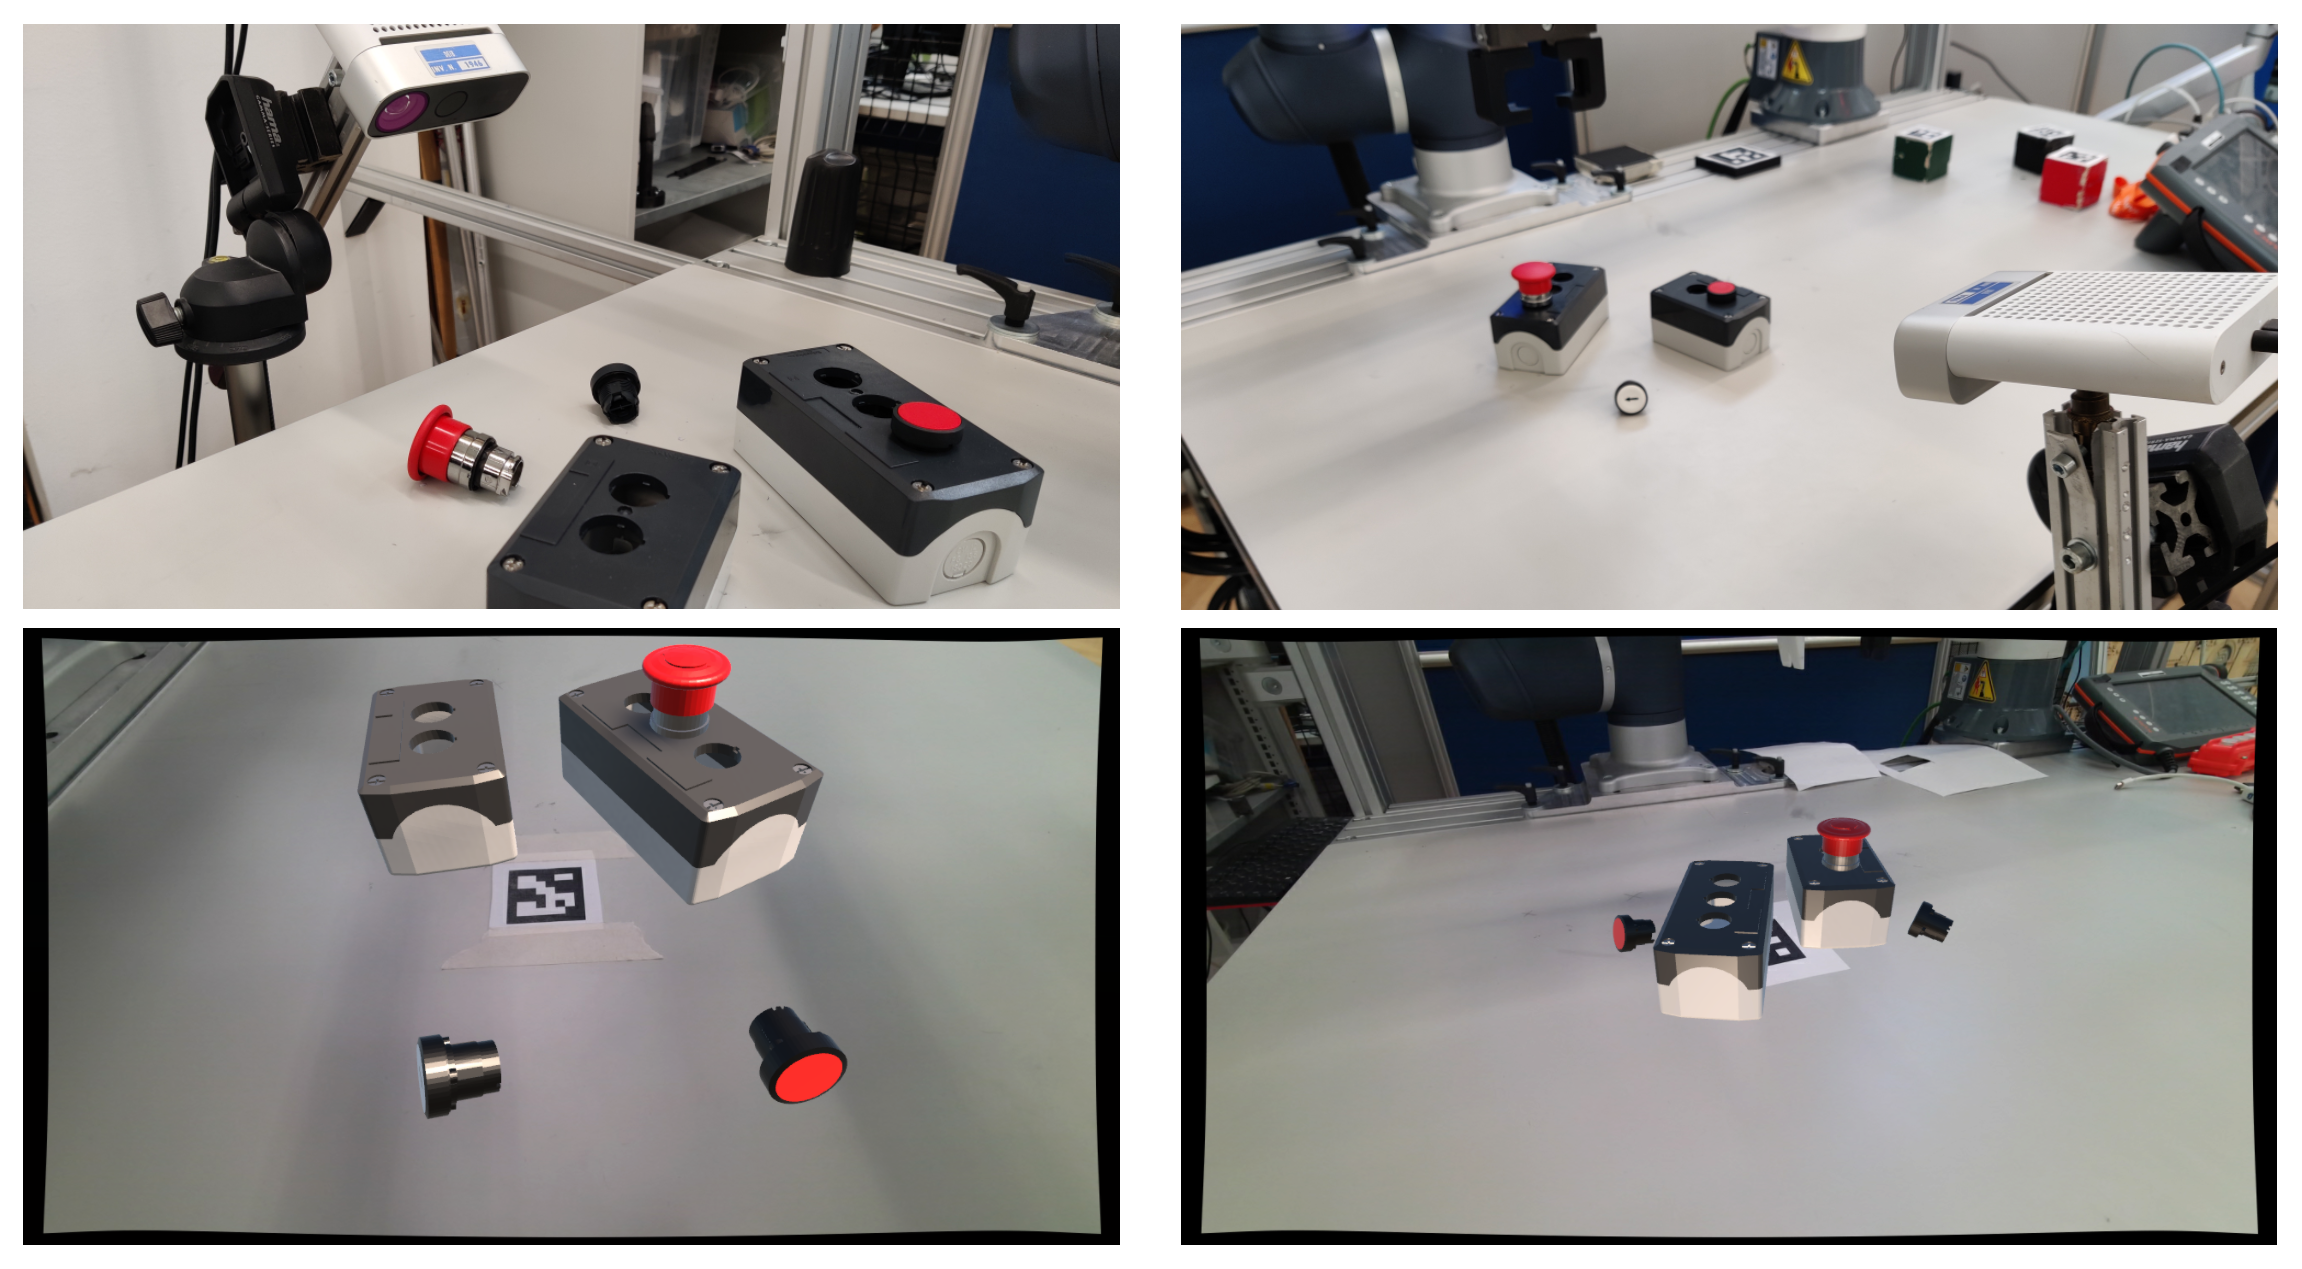
\includegraphics[width=\textwidth]{near_far.png}
    \caption{Photographs of the different capture positions for the ButtonPose-near (left) and ButtonPose-far (right) datasets, with a sample image presented for each.}
    \label{fig:near_vs_far}
\end{figure}

We can then compare the performance of the models trained on the two different datasets, shown in figure \ref{fig:near_vs_far_results}. As can be seen, the -near dataset obtained significantly better results than both the -far dataset and the regular dataset.

We can hypothesize that the reason for such a large gap between the two models lies in the input resolution of the network, which for $\phi = 0$ is set at 512 pixels. This makes it much more difficult for the network to make out fine details at a distance; in particular it would struggle to distinguish between the arrow button and the red button, since their faces would appear similar. This issue could therefore probably be alleviated by using higher values of $\phi$.

\subsection{False Positive Issues}
\label{false_positives_issue}

\begin{figure}[ht]
    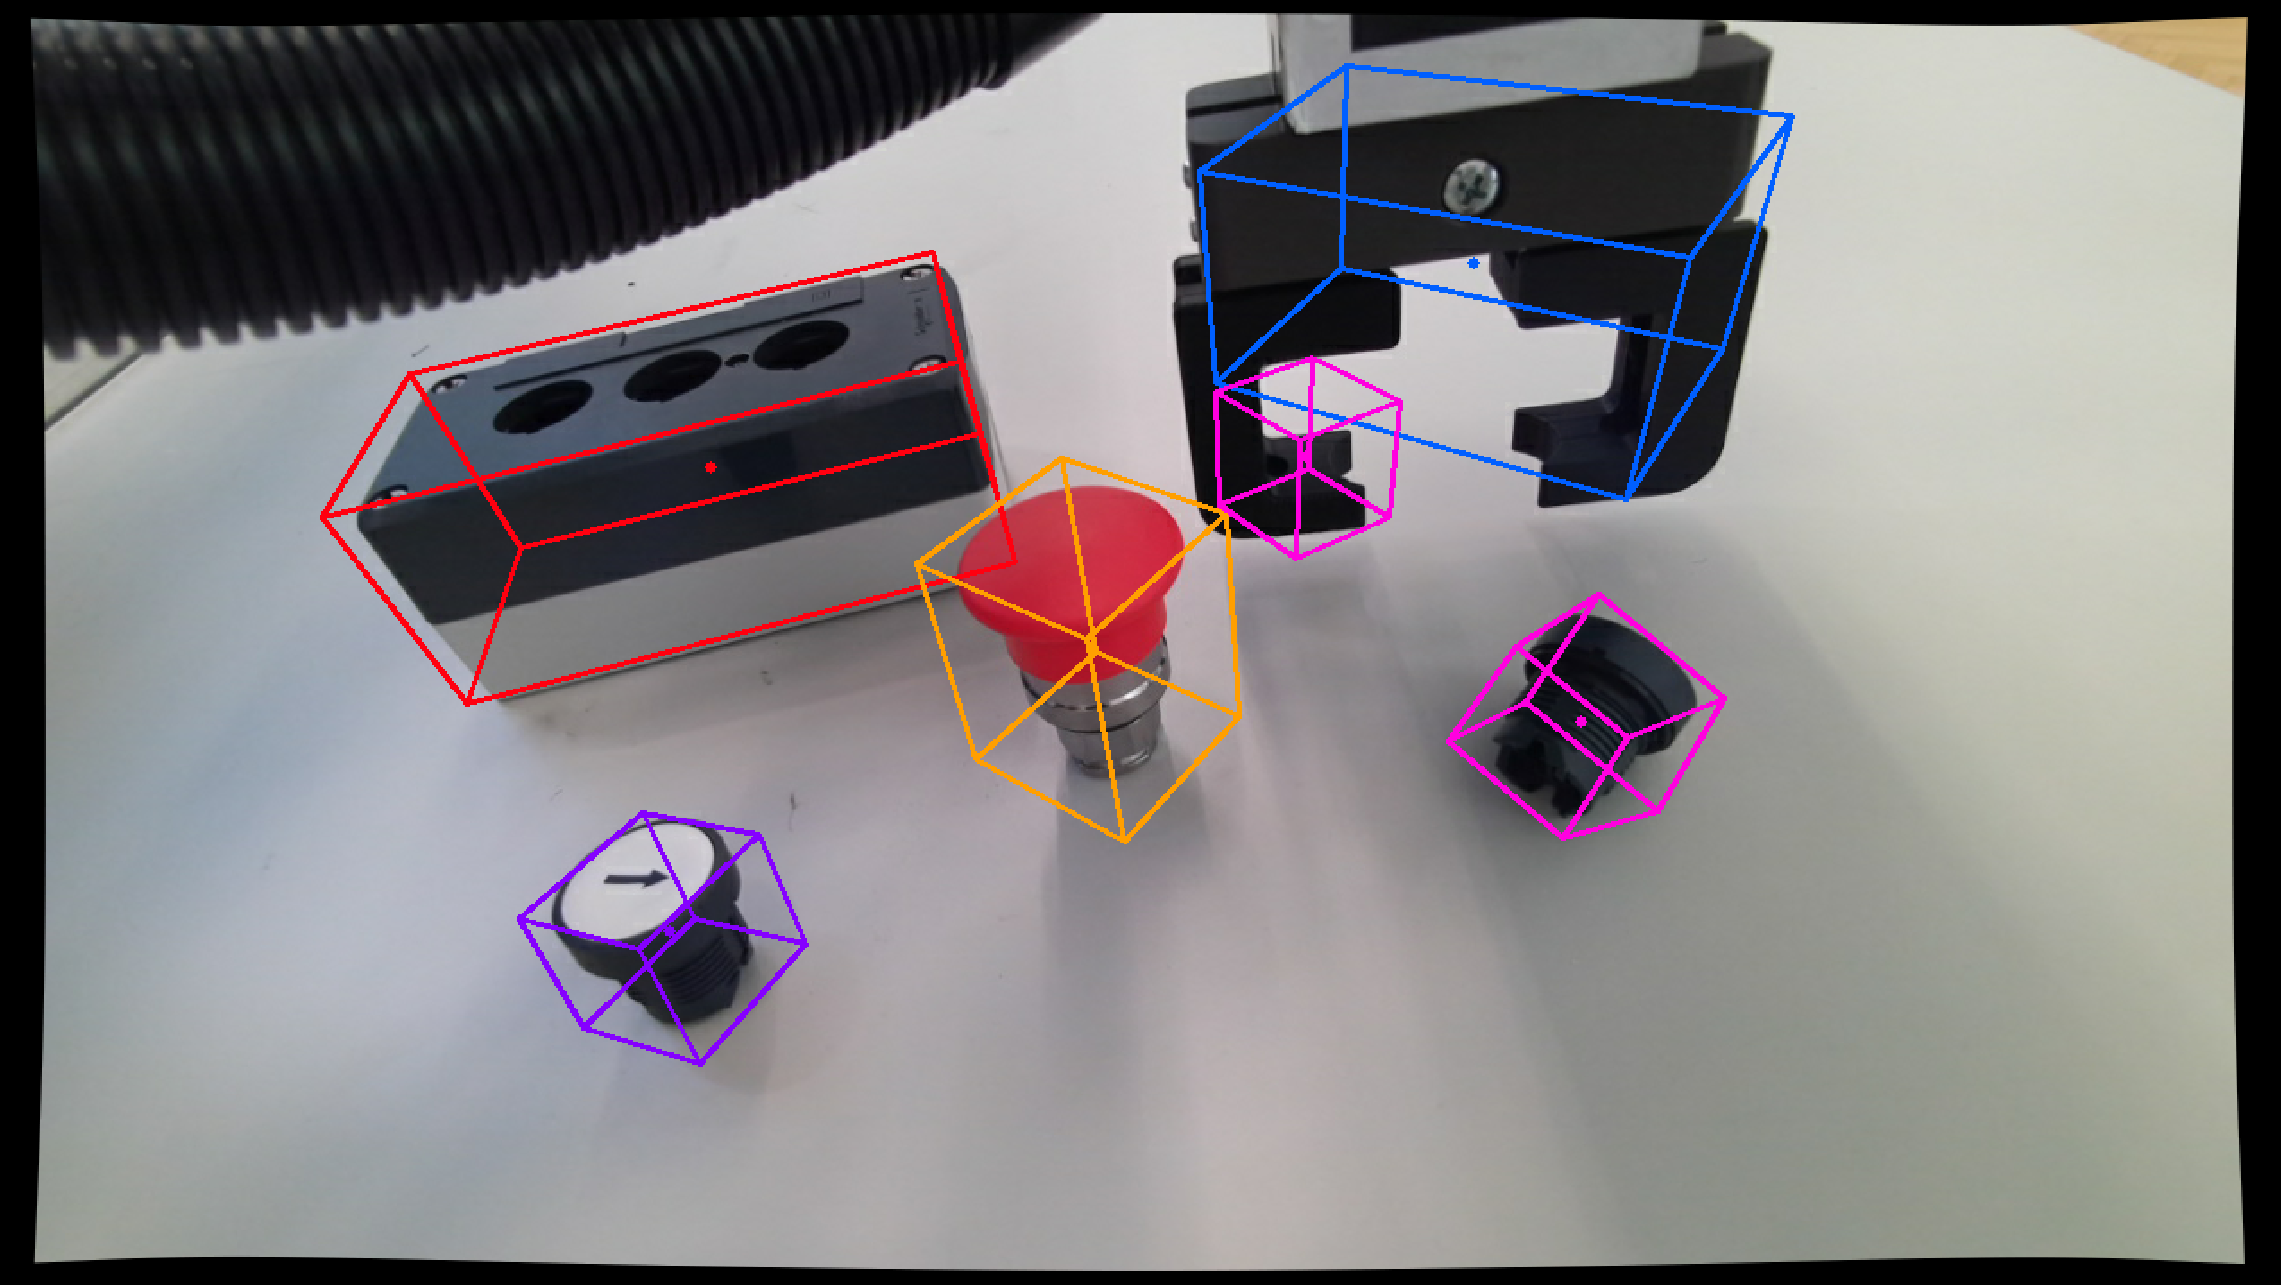
\includegraphics[width=0.7\textwidth]{false_positives.png}
    \caption{An example of how introducing untrained objects results in false positives.}
    \label{false_positives}
\end{figure}

A noticeable issue we encountered when testing our models in real world conditions was the difficulties they expressed in dealing with objects that are not present in the original dataset. In almost all cases, introduction of a never-before-seen object results in multiple false positives, as shown in figure \ref{false_positives}. This is because the model is not trained to "ignore" these objects, and thus attempts to classify them according to what it effectively "knows".

There are ways to approach and mitigate this issue. For example, if there is a high probability that a certain object that should not be tracked by the model will appear frequently in the scene, one could include that object within the dataset generation method without labelling it. In this manner, since the object would appear with a certain frequency during training, eventual false positives resulting from its presence would be recognized as such, and the model's behavior corrected.

We tested this method with the ScrewPose dataset: since all of its objects have a similar shape, a model trained on ScrewPose would tend to categorize any long and thin object as a screw, making it especially susceptible to false positives. However, introducing a "dummy" screw into most images, without labelling it as a dataset object, led to the model subsequently ignoring its appearance in most scenes. It was also able to generalise this behavior to a certain extent, ignoring other never-before-seen screws when they were introduced into the scene (see figure \ref{fig:inferencing}). Therefore in a case such as the one represented in figure \ref{false_positives}, if we were certain of the appearance of the gripper in many scenes, it would be worthwile to include its 3D model in some training images, so that the network could effectively learn to ignore it.

We hypothesize that by including a general enough set of "dummy" items in the training images, the model could then generalize this behavior to a wider variety of previously unseen objects. However, due to the nature of black-box methods, more research is necessary to verify whether this is feasible.

\section{Semantic Meaning Extraction Results}

In this section we will evaluate the performance of our semantic meaning extraction method. The precision-recall curves in figure \ref{fig:precisionrecall} were computed using the methodology described in section \ref{semantics_method_section} on the ButtonPose and ButtonPose-near datasets. The optimal thresholds and F1 scores are laid out in figure \ref{fig:optimal_F1}.

\begin{figure}[htp]
    \centering
    \subfloat[ButtonPose]{
        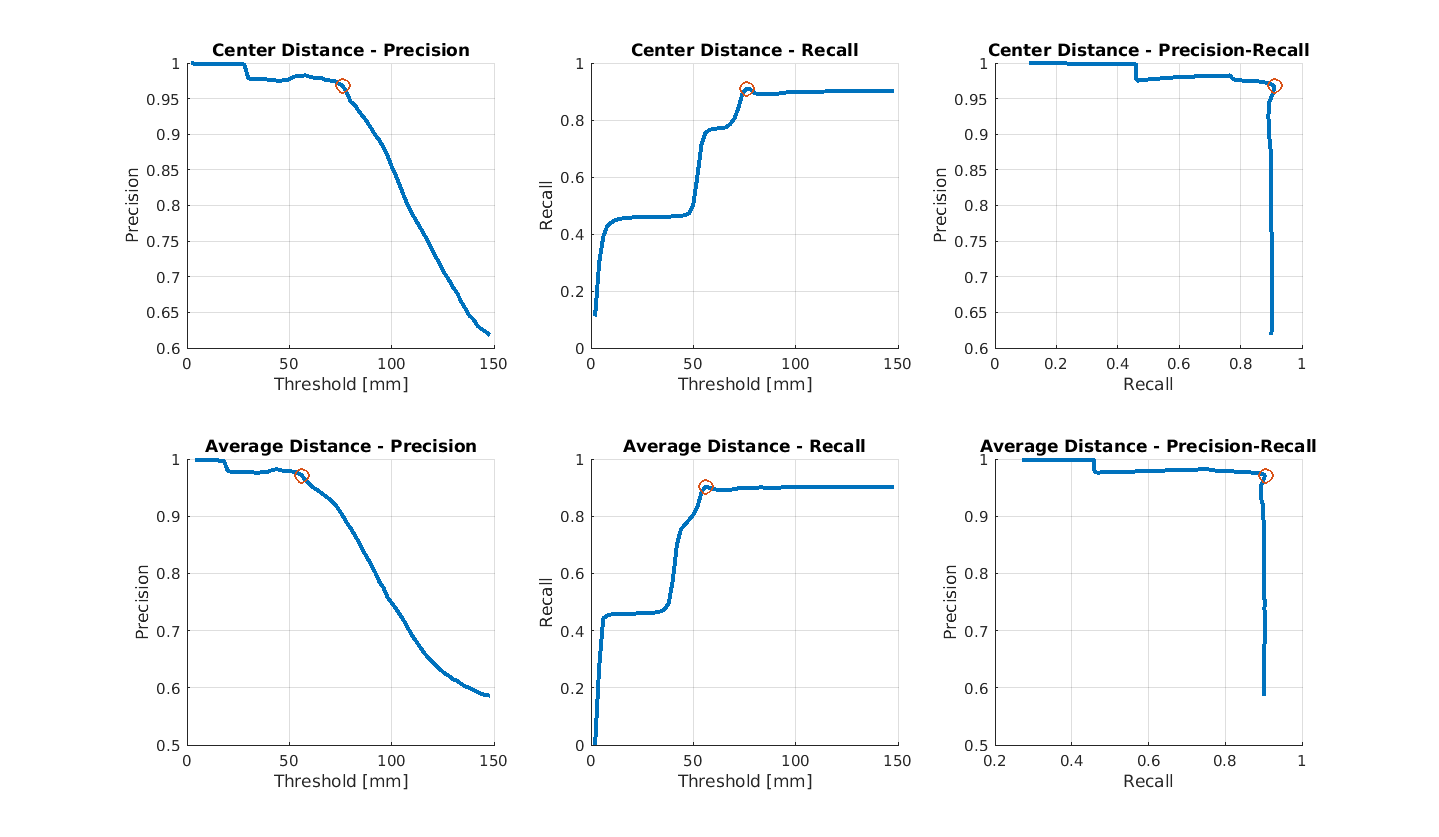
\includegraphics[width=\textwidth]{precision-recall.png}
    }

    \subfloat[ButtonPose-near]{
        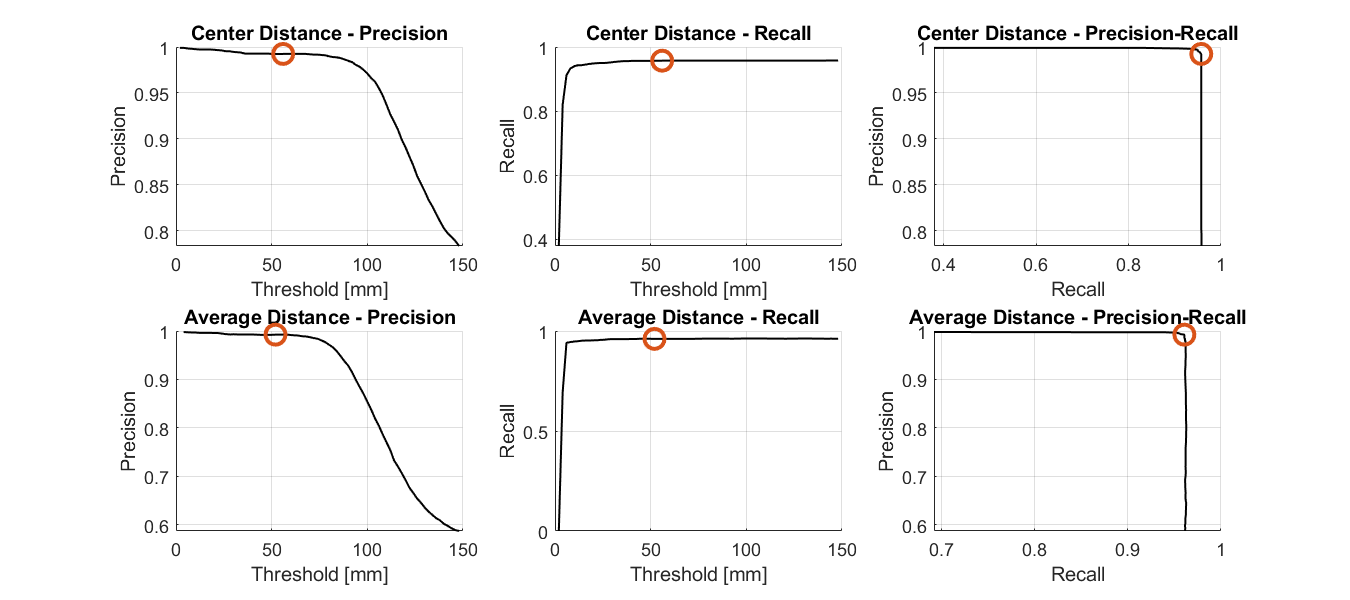
\includegraphics[width=\textwidth]{precision-recall_near.png}
    }
    
    \caption{Precision and recall for both distance metrics on the ButtonPose and ButtonPose-near datasets. The point with the best F1 score is highlighted with a red circle in both cases.}
    \label{fig:precisionrecall}
\end{figure}

\begin{figure}
    \subfloat[ButtonPose]{
        \begin{tabular}{|c||c|c|}
            \hline
            Metric & F1 & Threshold \\
            \hline \hline
            AD & 0.9369 & 56mm \\
            CC & 0.9255 & 78mm \\
            \hline
        \end{tabular}
    }
    \quad
    \subfloat[ButtonPose-near]{
        \begin{tabular}{|c||c|c|}
            \hline
            Metric & F1 & Threshold \\
            \hline \hline
            AD & 0.9763 & 52mm \\
            CC & 0.9746 & 56mm \\
            \hline
        \end{tabular}
    }
    
    \caption{Optimal F1 scores and thresholds for both the Average Distance (AD) and Center-to-Center (CC) metrics on the ButtonPose and ButtonPose-near datasets.}
    \label{fig:optimal_F1}
\end{figure}

Overall our method shows promising results, with precision-recall curves that are similar to the ideal, and high F1 scores.

We observe that our application obtained no great advantage in using Average Distance over Center-to-Center distance. Given the additional complexity and computation time, the increase in performance is not significant: for reference, computing the values for figure \ref{fig:precisionrecall} took 23.67 seconds using Center-to-Center, and 2650.34 seconds using Average Distance, making the second approximately 112 times slower.

We also obtained high values for the optimal \emph{distance thresholds}, above 5 cm in all testing conditions. We take this to mean that our method applies the threshold to determine whether a button is in a slot at all, while the slot itself is selected using the conflict resolution strategy previously described.

We hypothesize that the reason for this behavior lies in the dataset generation algorithm: by stating that the buttons can exclusively be either inside a slot or placed on the surface, we are in fact considering an ideal situation where a theoretical manipulator does not commit any errors in picking up and inserting the buttons. If failed attempts were considered in the dataset, it is likely that the optimal threshold would be lower, and the Average Distance method, being more sensible to situations with different rotations, would likely give better results than Center-to-Center.

Finally, the value of the threshold is also influenced by the probability distribution used for generating the poses for the button dataset, which in our case being a uniform distribution, resulted in a more spread-out placement, thus a higher optimal threshold. This is further compounded by the brute-force collision avoidance strategy implemented within the placement algorithm: if a placement attempt would generate an intersection with an already placed object, the placement is simply re-attempted from scratch. This naturally results in less conditions where dataset objects are in close proximity, and therefore in a higher threshold.

\section{Real-World Application Results}

As previously described in section \ref{semantics_method_section}, we tested the performance of our vision method in a real-world application where the robot had to pick up a button from the ButtonPose dataset and insert it into a slot on one of the button boards. while relying solely on RGB images.

\begin{table}
    \begin{center}
        \begin{tabular}{|c|cc|}
            \hline
            Button Type & Small & Large \\
            \hline
            Total Attempts & 10 & 10 \\
            \hline
            Successful Pick-Ups & 7 & 10 \\
            \hline
            Successful Insertions & 5 & 7 \\
            \hline

        \end{tabular}
    \end{center}
\end{table}

In our testing, the robot was able to pick up the smaller buttons seven times out of ten, while it was able to pick up the larger button in all test cases. Out of the times it was able to pick up a button, the following insertion was performed correctly in 72\% of cases.

The main issue encountered during testing was the prevalence of small errors in the rotation of the gripper relative to the button. These errors are usually in the neighborhood of $\pm5\degree$, but they are noticeable and can lead to mistakes, as the button may be gripped in an awkward manner.

\begin{figure}[ht]
    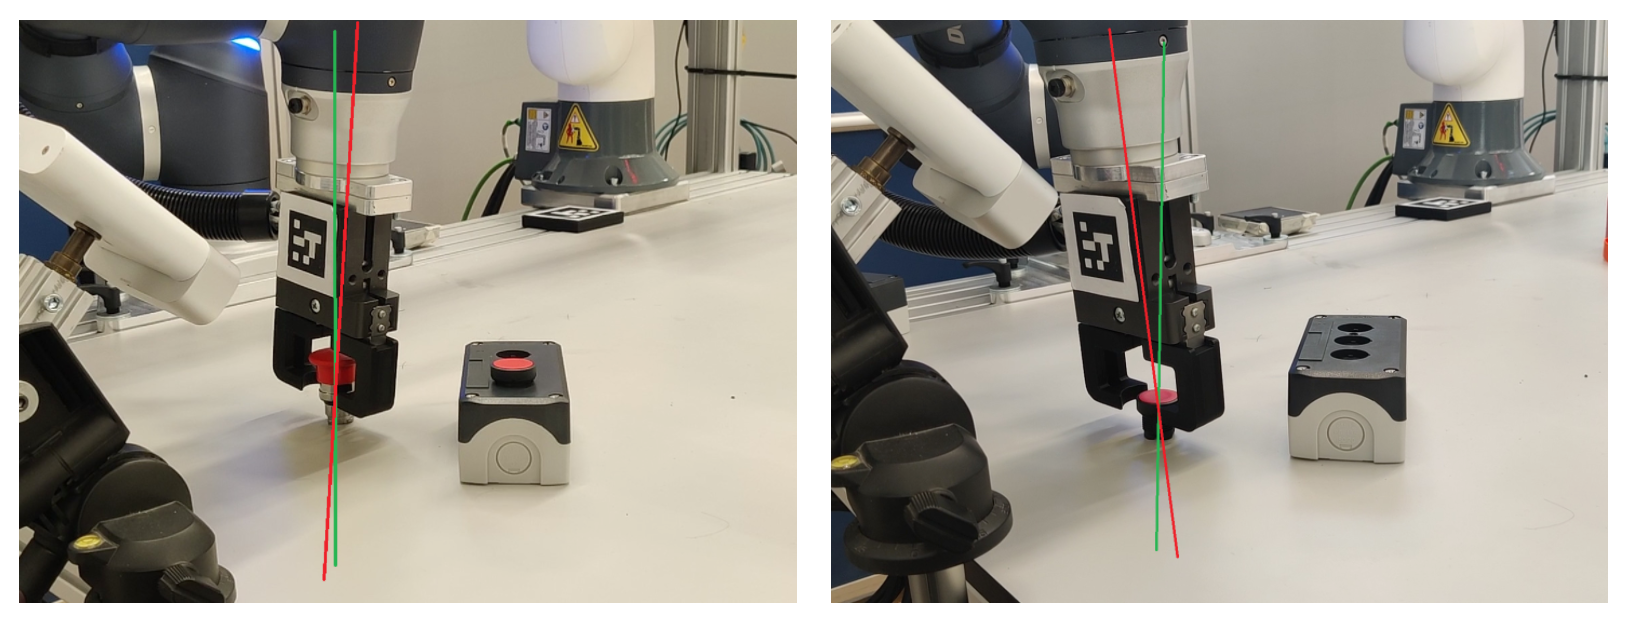
\includegraphics[width=\textwidth]{roboterrors.png}
    \caption{Examples of small rotation errors when attempting to pick up a button with the robotic arm. The green line indicates the button's central axis, while the red line is the robot's.}
\end{figure}

Positioning relative to the boards was instead very accurate, and errors is the insertion phase were mostly due to mistakes in grasping the necessary buttons.

Overall the robot performed much better when dealing with the larger buttons and boards than when dealing with the smaller buttons, making its reliability very dependant on the accuracy of the pose estimation network. The network proved to be relatively accurate regarding the 3D position of objects, but often not as accurate regarding their rotation, leading to small mistakes that overall may have negative effects on tasks requiring high precision.
